\section{Experiments}

\subsection{Testing overlay alternatives}
In this section we evaluate the methods described in section \ref{sec:alternative_methods}.  We used the top 8 states from the Census Track Datasets to evaluated the alternatives.  It measures the execution time of the overlay at the master/root node (`At master/root' tag), repartition by segment's label (`By label' tag) and performing an intermediate step at a given level (`At level [X]' tag, where X is the level given by the user).  Figure \ref{fig:overlay_tester} shows the results of the testing.  It clearly shows that the overlay by label repartition gives the best results in all the tests.

\begin{figure}[!ht]
    \centering
    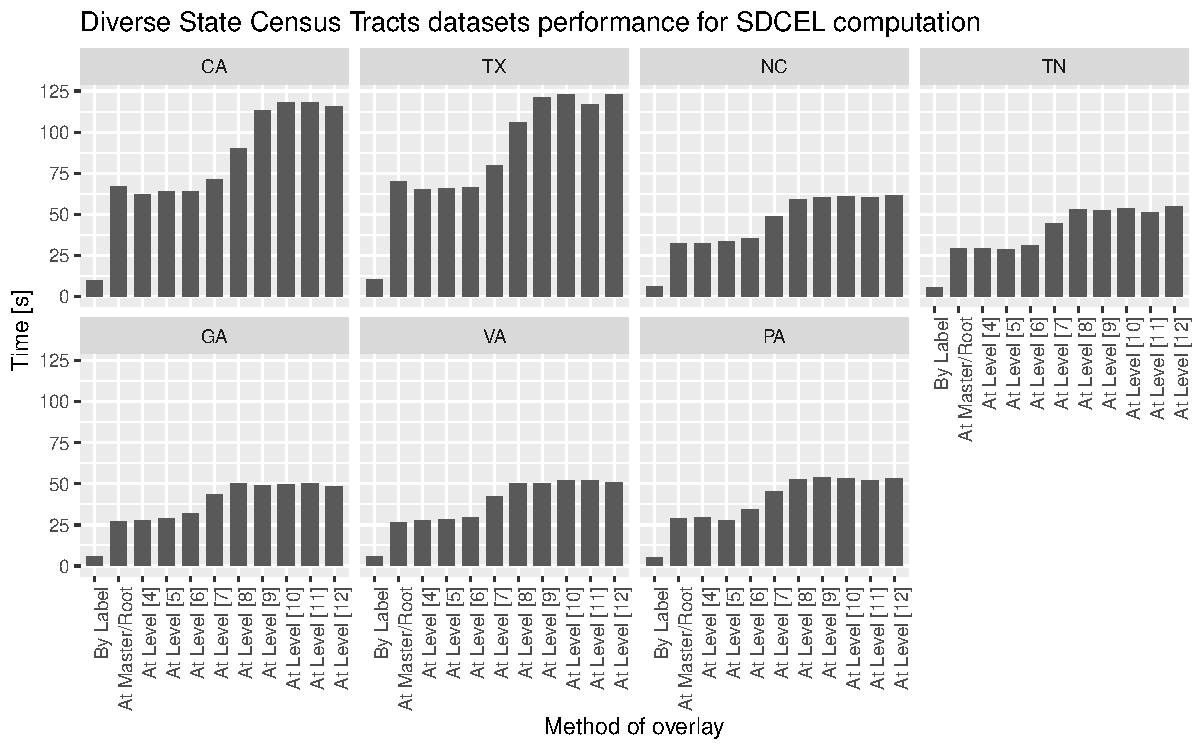
\includegraphics[width=\linewidth]{figures/experiments/Overlay_Tester}
    \caption{Overlay methods evaluation.}\label{fig:overlay_tester}
    \Description[Overlay methods evaluation]{This figure shows the overlay methods evaluation.}
\end{figure}

\subsection{Real datasets}
In order to test our implementation, we used two datasets of polygons.  The first one is the California Census-Track Administrative Levels - CCTAL. The layer A collects the census tracts in California during 2000 meanwhile the layers B collects those ones for 2010.  Something to note with this dataset is that the differences between the layers no just show the changes in time but also they present a small gap (due to technical reasons) between the polygons which will increase considerably the number of intersections and new faces the DCEL should be able to identify.

The second dataset is from the Global Administration Areas - GADM\footnote{\url{https://gadm.org/}}. It collects geographical boundaries of the countries and their administrative divisions around the globe.  For the tests, we select the levels 0 (Countries) and level 1 (States). We take individual polygons, it is, any multi-polygon was divided and each polygon was manage independently. The details of both datasets are summarized in table \ref{tab:datasets}.  Experiments runs on a cluster of 12 nodes running Apache Spark 2.4.  Each node has 9 cores and 12G memory available.

\begin{table}[!ht]
    \caption{Datasets details.}
    \label{tab:datasets}
    \begin{tabular}{c c c c}
        \toprule
        Dataset & Layer & Number        & Number    \\
                &       & of polygons   & of edges  \\
        \midrule
        CCTAL & Polygons for 2000 & 7028 & 999763  \\
              & Polygons for 2010 & 8047 & 2901758 \\
        GADM  & Polygons for Level 0 & 116995 & 32789444 \\
              & Polygons for Level 1 & 117891 & 37690256 \\
        \bottomrule
    \end{tabular}
\end{table}

\subsection{California dataset}

The first set of experiments aim to compare the performance of the SDCEL implementation over the CCTAL Dataset varying the number of partitions used to divide the data. It sets the parameters of the quadtree used to split the data to obtains different values from coarse (100) to fine (15K) number of partitions (left part in figure \ref{fig:ca}).  Clearly there are a trade-off in this case.  The more partitions, each subdivision will have to deal with a smaller number of edges will means a faster execution.  However, it the number of partitions is too high, the cost to divide and collect the results will have an impact.  We can see that an optimal value can be reached around 7K partitions.  A zoom of this part of the plot is shown in figure \ref{fig:ca}.

In addition with the partition analysis, we compare the performance of the SDCEL implementation against the sequential solution offered by the CGAL library.  The independent column in the right of figure \ref{fig:ca} shows its execution time.  Clearly, the appropriate setting for the number of partitions of SDCEL can beat the sequential implementation by several orders of magnitude.

\begin{figure}[!ht]
    \centering
    \subfloat[SDCEL vs CGAL. \label{fig:ca_a}]{%
        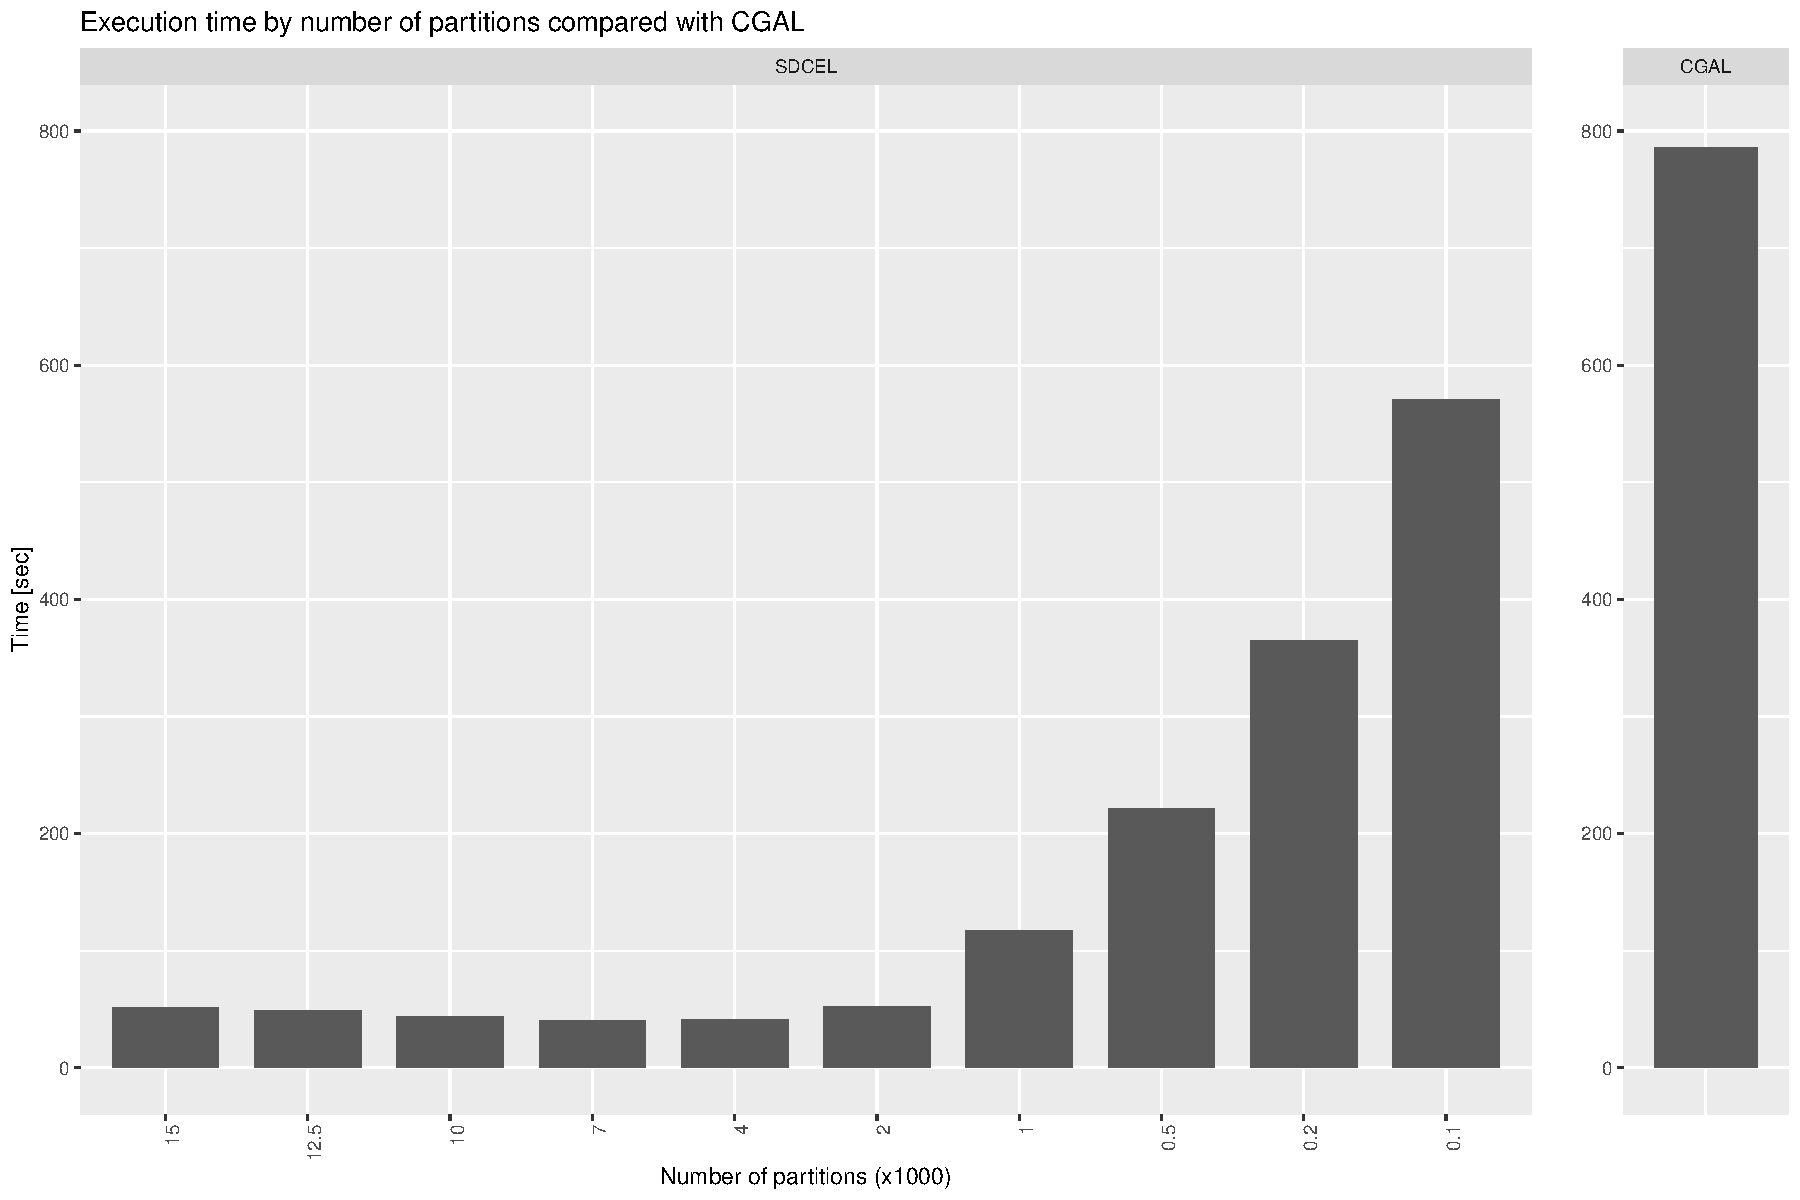
\includegraphics[width=0.45\linewidth]{figures/experiments/ca.pdf}}
    \hfill
    \subfloat[Focus on the most relevant number of partitions. \label{fig:ca_b}]{%
        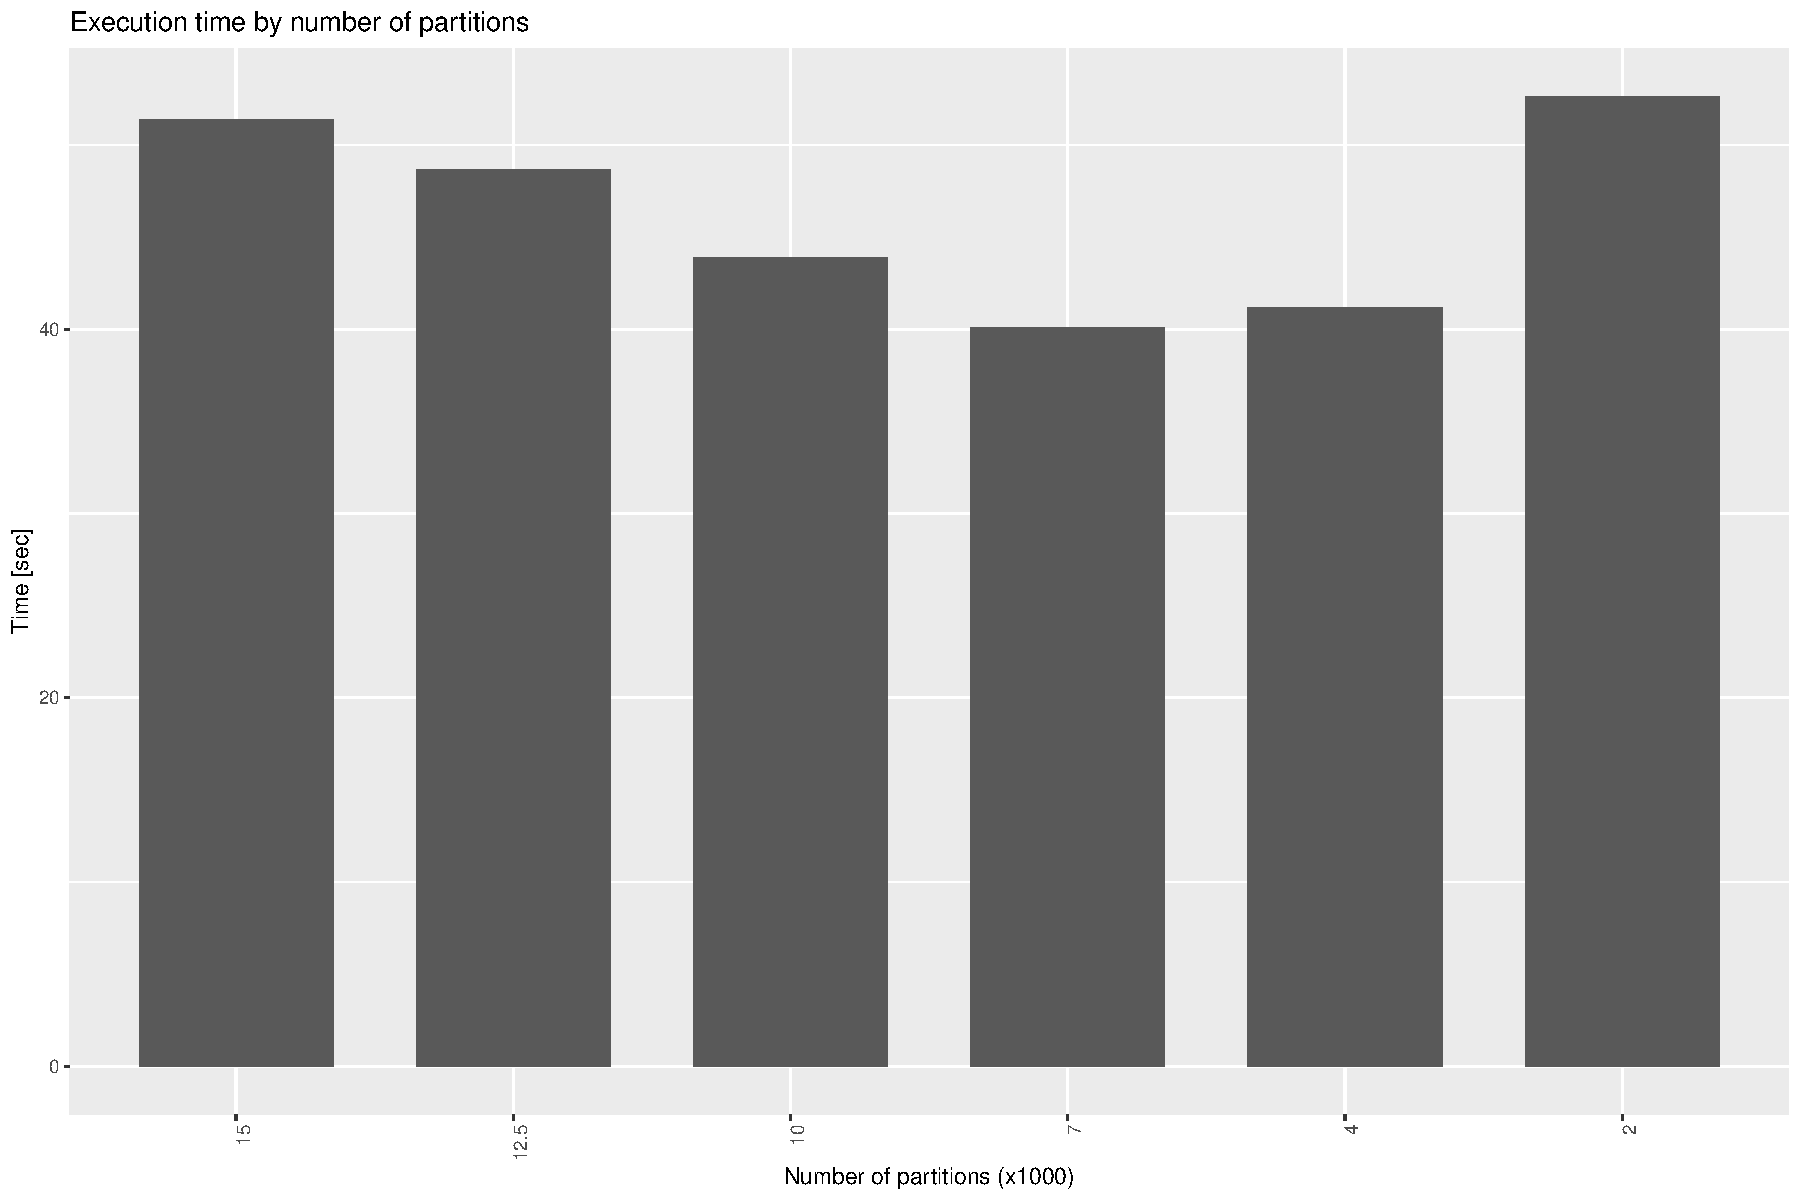
\includegraphics[width=0.45\linewidth]{figures/experiments/ca_sample.pdf}}
    \caption{Experiments with CCTAL dataset. \label{fig:ca}} 
    \Description[Experiments with the CCTAL dataset]{This figure shows the experiments using the CCTAL dataset.}
\end{figure}

\subsection{GADM dataset}

\begin{figure}[!ht]
    \centering
    \subfloat[SDCEL execution time. \label{fig:gadm_a}]{%
        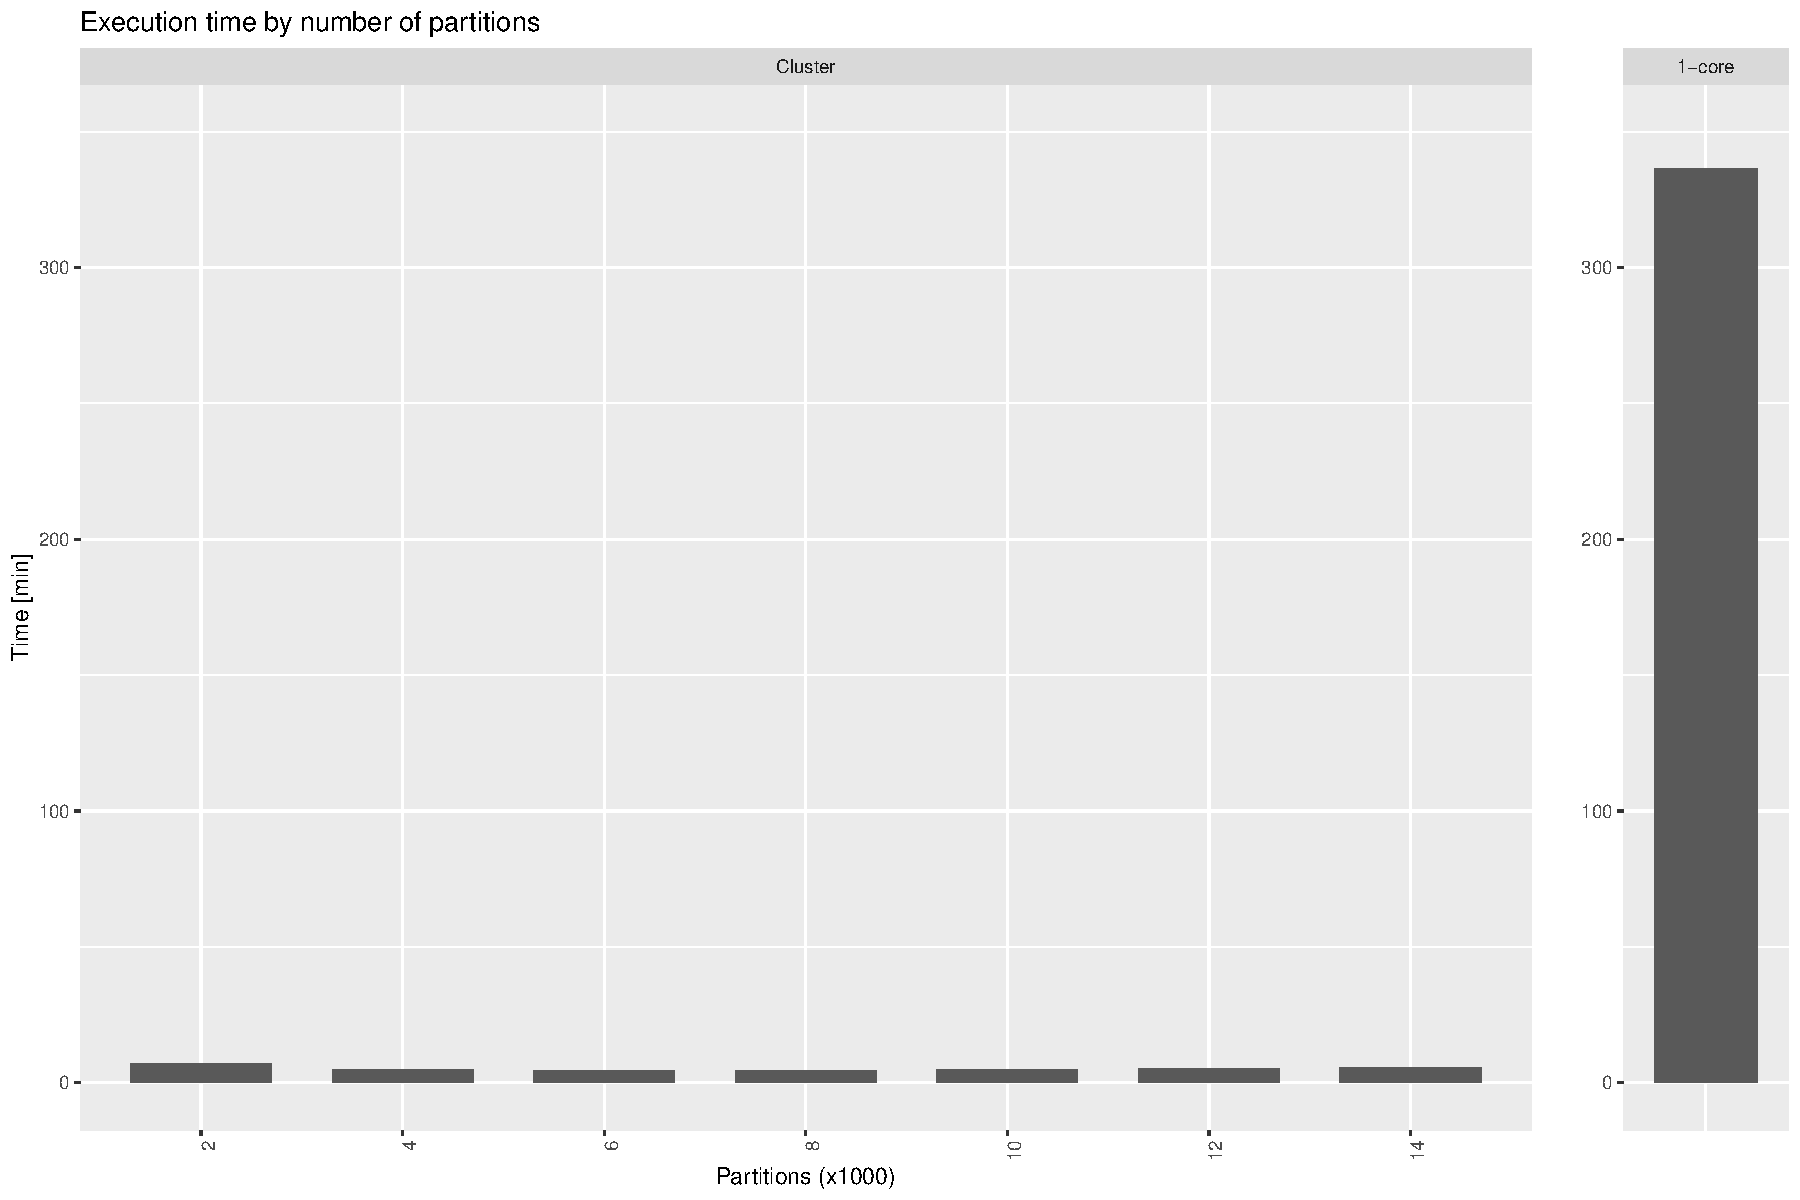
\includegraphics[width=0.45\linewidth]{figures/experiments/gadm.pdf}}
    \hfill
    \subfloat[Focus on the most relevant number of partitions. \label{fig:gadm_b}]{%
        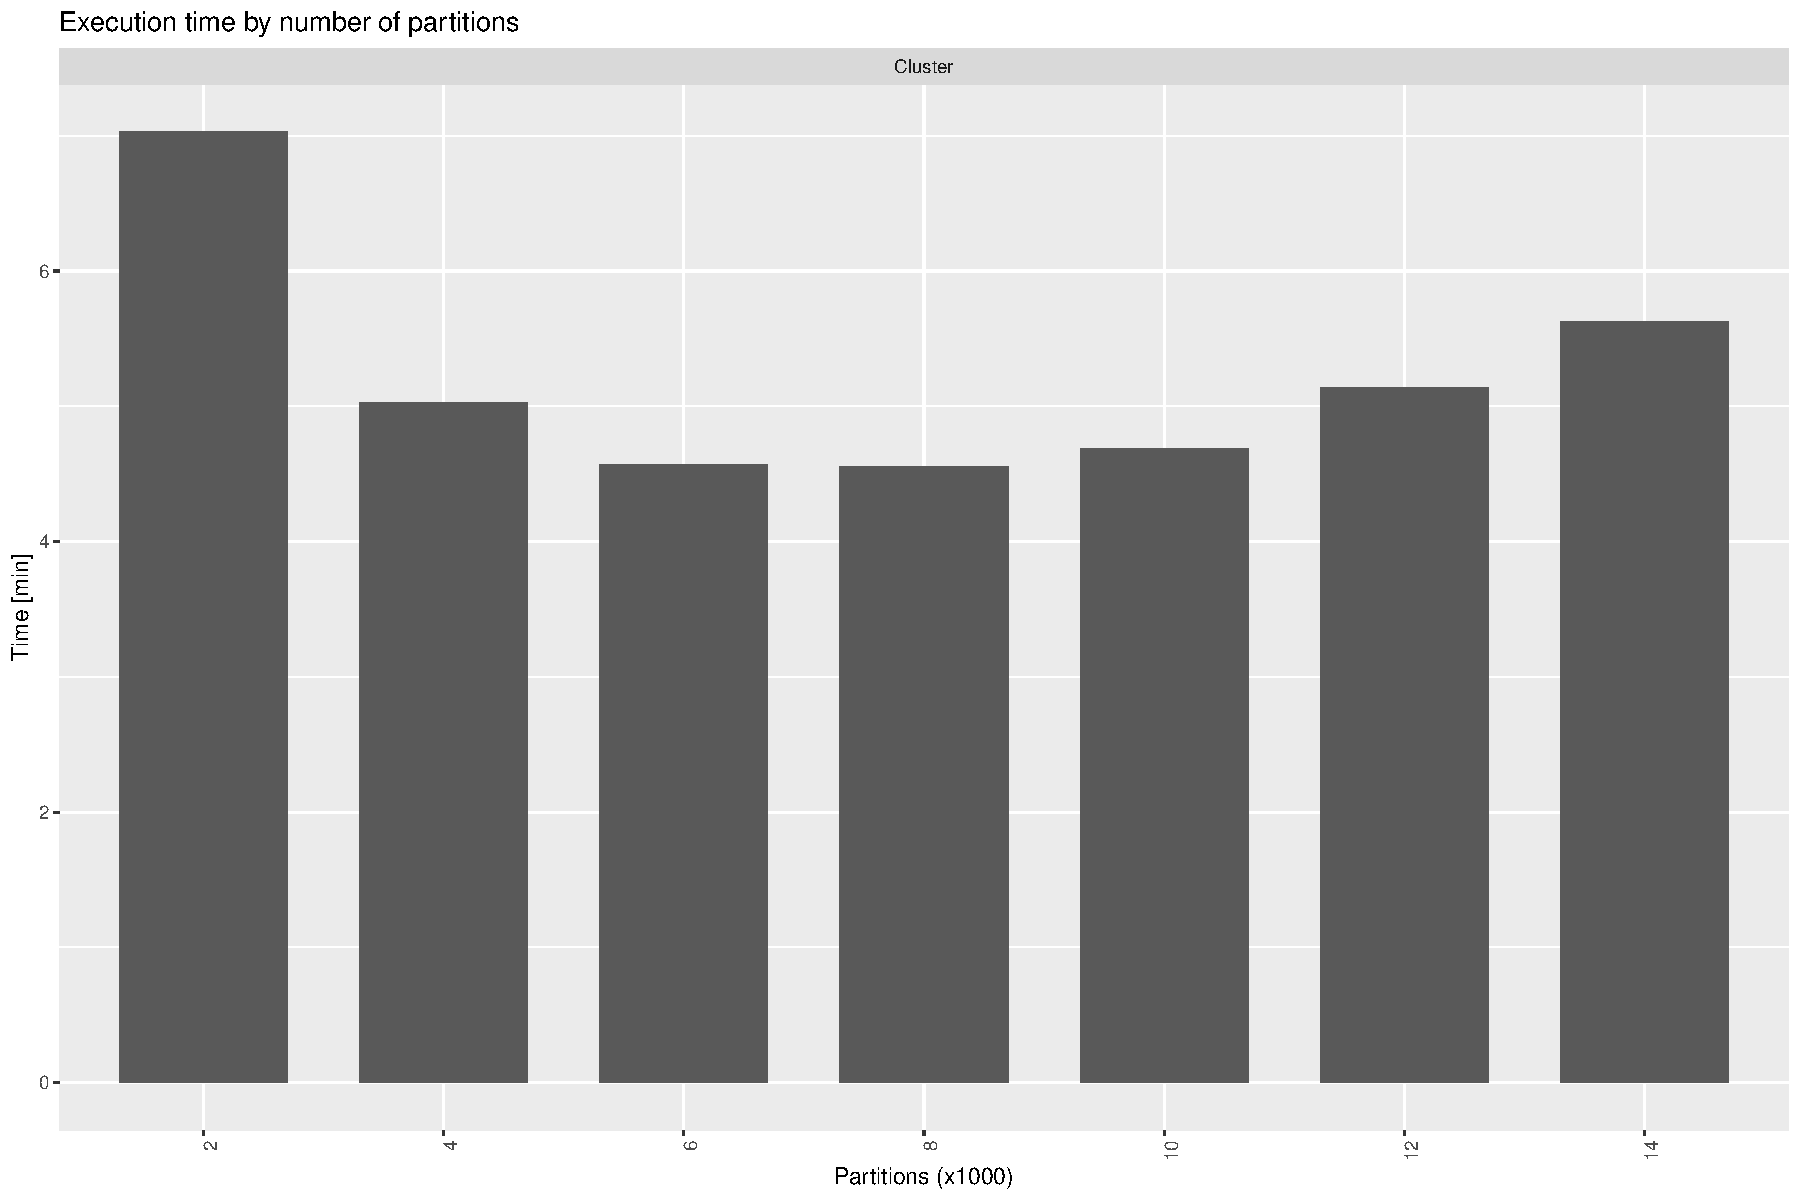
\includegraphics[width=0.45\linewidth]{figures/experiments/gadm_sample.pdf}}
    \caption{Experiments with GADM dataset. \label{fig:gadm}} 
    \Description[Experiments with the GADM dataset]{This figure shows the experiments using the GADM dataset.}
\end{figure}

The CCTAL dataset is relatively small but useful in order to compare with the sequential alternative.  However, the CGAL library is unable to deal with big spatial data.  For the case of the GADM dataset, we only present the results for SDCEL given that CGAL crash when run this volume of data.  Figure \ref{fig:gadm} show the execution time of SDCEL varying the number of partitions.  We can seen a similar trade-off as with CCTAL dataset which can be seen more clearly in the right of the figure.  We can identify a optimal number of partitions around the 6K -8K partitions.  Similar as before, the independent column at the right of figure \ref{fig:gadm} shows the comparison if the SDCEL runs using just one core.

\subsection{Speed up and scale up analysis}

Finally we analyze the scalability of the implementation through the speed up and scale up tests.  For the speed up, the GADM dataset was used with different amount of resources, in this case the number of available nodes.  Each time, the nodes were duplicated and the performance was measured.  Figure \ref{fig:speedup} shows  how as resources double, the response time is almost cut in half each time, as it is expected.  

In the case of the scale up test, the workload was also modified.  The GADM dataset was split in 4 regions slightly similar in the number of edges they collect.  At each iteration, both the size of the data and the amount of available resources were doubled. As it was expected, the performance at each scenario should not change significantly as it is shown in figure \ref{fig:scaleup}.

\begin{figure}[!ht]
    \centering
    \subfloat[Speed Up \label{fig:speedup}]{%
        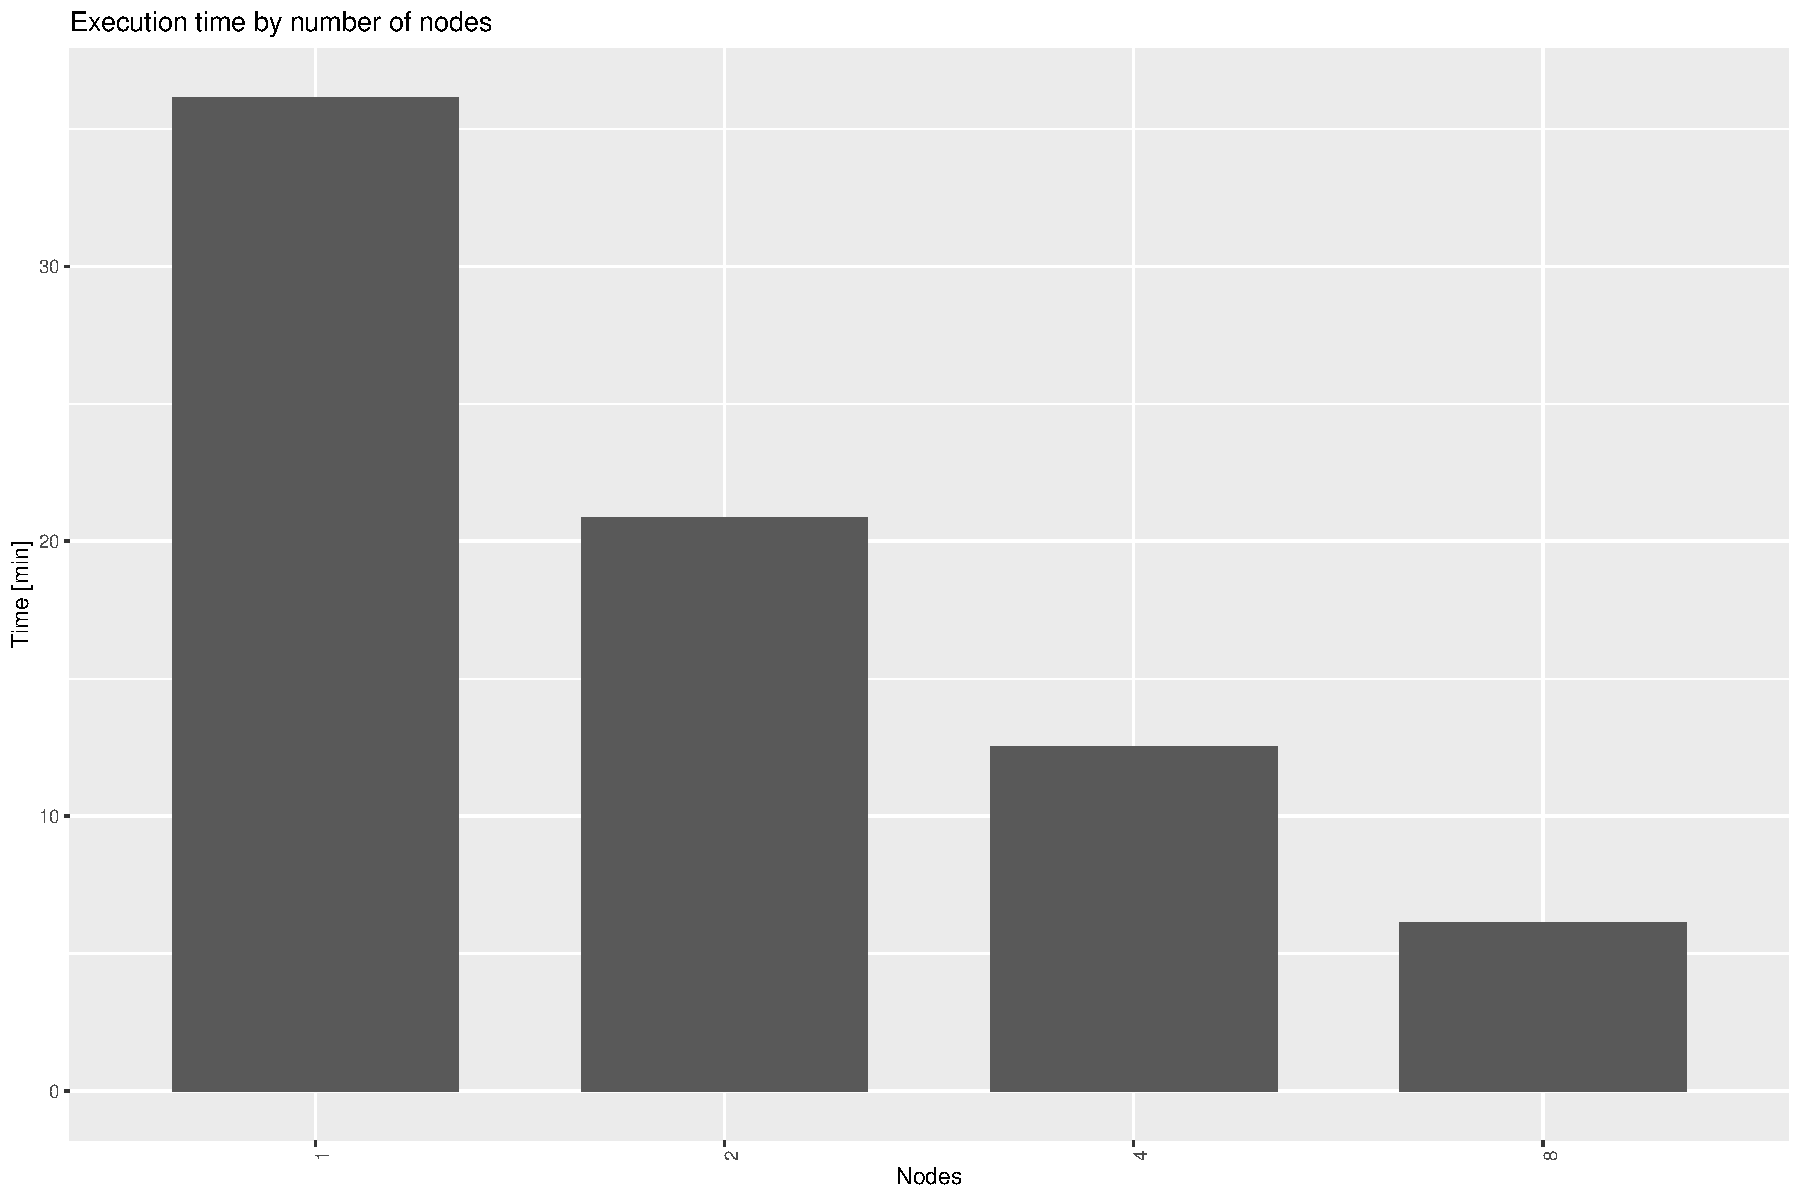
\includegraphics[width=0.45\linewidth]{figures/experiments/speedup.pdf}}
    \hfill
    \subfloat[Scale Up \label{fig:scaleup}]{%
        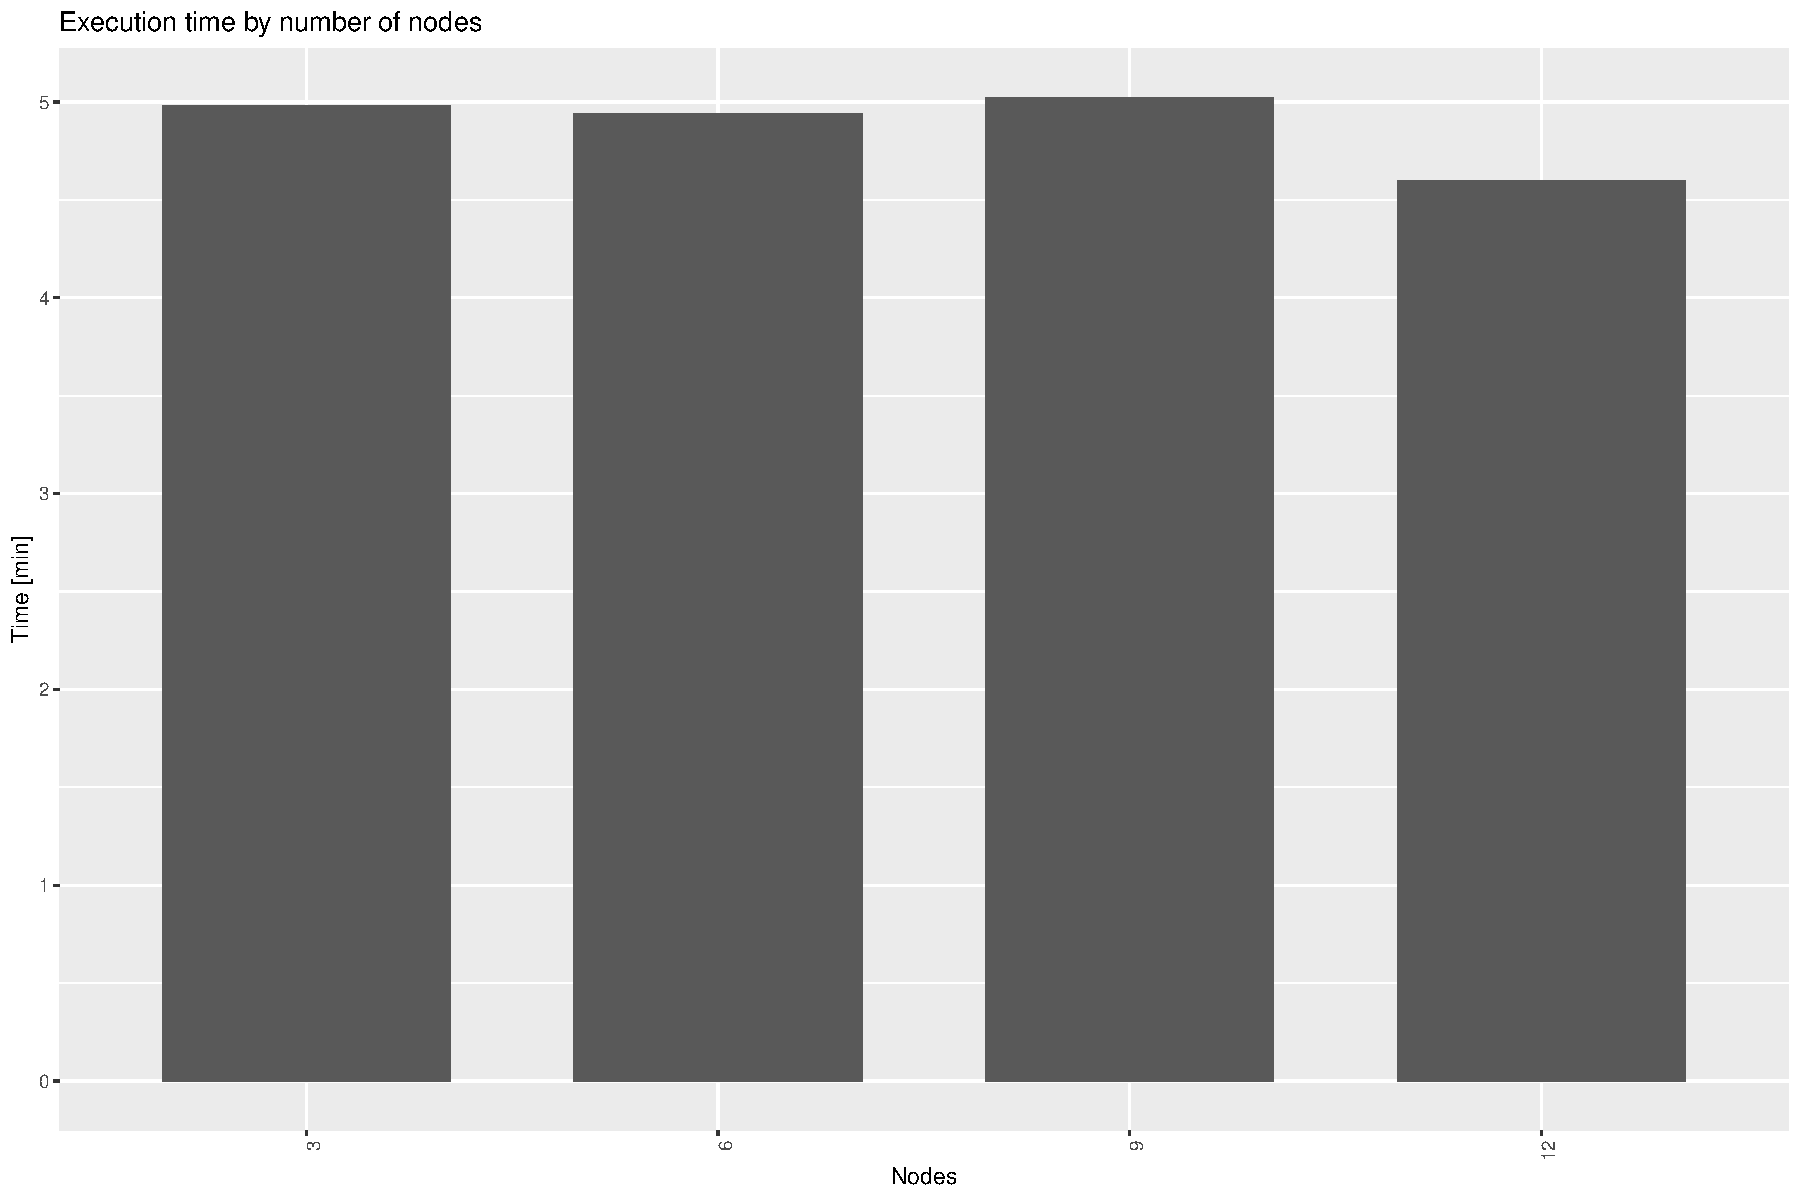
\includegraphics[width=0.45\linewidth]{figures/experiments/scaleup.pdf}}
    \caption{Speed Up and Scale Up experiments.} \label{fig:speed_scale} 
    \Description[Speed Up and Scale Up experiments]{This figure shows the experiments for speed up and scale up analysis.}
\end{figure}
